\documentclass{../../fal_assignment}
\graphicspath{ {../../} }

\usepackage{enumitem}
\setlist{nosep} % Make enumerate / itemize lists more closely spaced
\usepackage[T1]{fontenc} % http://tex.stackexchange.com/a/17858
\usepackage{url}
\usepackage{todonotes}

\title{Hacking Hardware}
\author{Brian McDonald and Alcwyn Parker}
\module{COMP140 \& GAME160}

\begin{document}
	
	\maketitle
	
	\section*{Introduction}
	
	\begin{marginquote}
		Hacker definition: ``A person who enjoys exploring the details of programmable systems and stretching their capabilities, as opposed to most users, who prefer to learn only the minimum necessary.''
		
		--- Jargon File
		
	\end{marginquote}
	\marginpicture{flavour_pic}{
	    Arduino is an open-source prototyping platform based on easy-to-use hardware and software.
	}
	
	In this assignment you will work as an individual to design a game which supports a novel alternative controller. In addition to this, you will also develop your Object Orientated Skills by creating a version of Pong which can be played with a Custom Controller
	
	Experimentation, ingenuity, and creativity are at the heart of everything that professional game developers do. To this end, building your own custom game controller is the perfect place to exercise these characteristics. However, you will also gain invaluable exposure to working with computer hardware. In recent years, there has been considerable growth in the development of new fabrication technologies, such as 3D printers. In addition, electronics, from primitive transistors to complex computer chips, have all become much cheaper. Accessibility to these tools has, therefore, unveiled an unprecedented opportunity to invent and innovate in this space. Increasingly, app developers are augmenting mobile software with new wearable devices, and so to will game developers with the advent and increasing popularity of augmented reality games.
	
	This assignment is formed of several parts:
	
	\begin{enumerate}[label=(\Alph*)]
		\item \textbf{Write}, a proposal for a game that uses an alternative controller which contains:
		\begin{enumerate}[label=\roman*.]
			\item \textbf{describe} the game
			\item \textbf{describe} the core game mechanics
		\end{enumerate}
		\item \textbf{Write} a proposal for an alternative controller which contains: 
		\begin{enumerate}[label=\roman*.]
			\item \textbf{research} into existing alt-Controllers
			\item \textbf{description} of the physical controller
			\item \textbf{design} of physical controller
		\end{enumerate}
		\item {Develop} a version of Pong which can be controlled using a custom controller
		\begin{enumerate}[label=\roman*.]
			\item \textbf{demonstrate} your understanding of the Ardunio Platform
			\item \textbf{revise} your proposal for your game and controller
		\end{enumerate}
		
	\end{enumerate}
	
	\subsection*{Assignment Setup}
	
	Fork the GitHub repository at:
	
	\indent \url{https://github.com/Falmouth-Games-Academy/comp140-gam160-game}
	
	Use the existing directory structure and, as required, extend this structure with sub-directories. Ensure that you maintain the \texttt{readme.md} file.
	
	Modify the \texttt{.gitignore} to the defaults for \textbf{Unity} or \textbf{Unreal}. Please, also ensure that you add editor-specific files and folders to \texttt{.gitignore}. 
	
	\subsection*{Part A}
	
	Part A consists of a \textbf{single formative submission}. This work will be assessed on a \textbf{threshold} basis. The following criteria are used to determine a pass or fail:
	
	\begin{enumerate}[label=(\alph*)]
		\item Submission is timely;
		\item Choice of game is feasible;
		\item Design is distinctive and has creative merit.
	\end{enumerate}
	
	To complete part A, write your proposal in the \texttt{readme.md} document. This should use the \textbf{markdown} syntax, for additional guidance, please read the following  
	
	\indent \url{https://github.com/adam-p/markdown-here/wiki/Markdown-Cheatsheet}
	
	Please make a pull request before \textbf{Friday 9th of February at 5pm}, you will receive immediate feedback from your tutor. 
	
	\subsection*{Part B}
	
	Part B is formed of \textbf{single formative submissions}. This will be assessed on a \textbf{threshold} basis. The following criteria are used to determine a pass or fail:
	
	\begin{enumerate}[label=(\alph*)]
		\item Submission is timely;
		\item Research activities are exhaustive and well referenced
		\item Description of the controller 
		\item Design is distinctive and has creative merit.
	\end{enumerate}
	
	To complete Part B, write your proposal in the \texttt{readme.md} document using markdown syntax.
	
	Please make a pull request before \textbf{Friday 16th of February at 5pm}, you will receive immediate feedback from your tutor. 
	
	\subsection*{Part C}
	
	Part C is a \textbf{single summative submission}. This work is \textbf{individual} and will be assessed on a \textbf{criterion-referenced} basis. Please refer to the marking rubric at the end of this document for further detail.
	
	You will use an Arduino to create a game controller for the retro arcade classic, Pong. The source for the game exists already. You are tasked with modifying the code to include bidirectional communication with the Arduino. The suggested design of the final controller is: two potentiometers to control the paddles and some combination of LEDs that flash when someone scores. Feel free to add some creative flair to the suggested design or modify it completely. The only requirement is that there must be two-way communication between the Arduino and the game. The wiring diagram below shows a potential controller setup for this worksheet. You are encouraged to create the controller one step at a time following the steps below. \textbf{DO NOT} wire everything up in one go and then expect it to work first time. 
	
	\begin{figure}[!ht]
		\begin{center}
			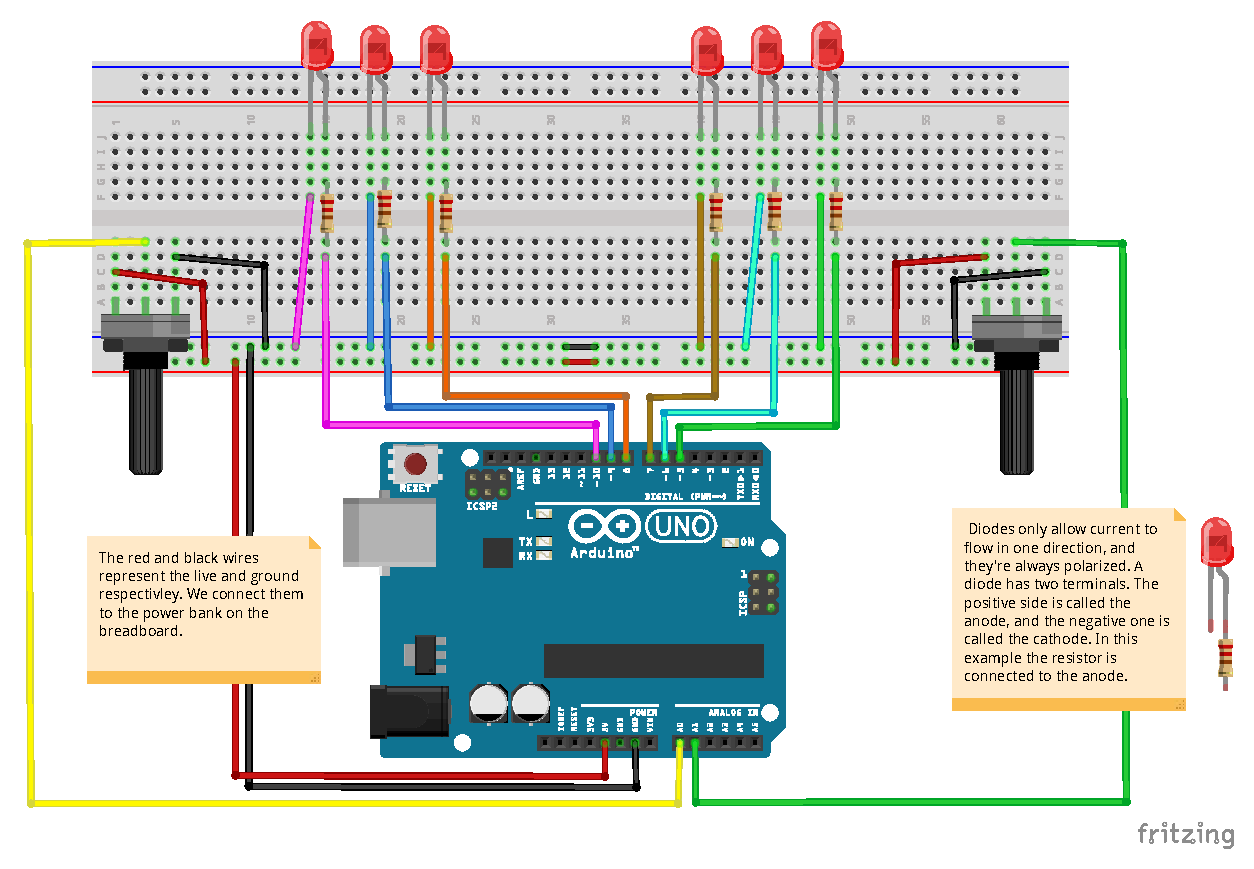
\includegraphics[width=0.9\textwidth]{assets/arduino-pong.pdf}
		\end{center}
		\caption{Pong Controller Wiring Diagram}
		\label{fig:wiring}
	\end{figure}
	
	\section{A Single Potentiometer} \label{arduino-first}
	To begin, connect one potentiometer to the breadboard. Hook the potentiometer up to the Arduino. Then write an Arduino sketch to send the potentiometer values over the serial connection. Tested this works using the serial monitor built into the Arduino IDE. Then, adapt the Pong source to update player one's paddle using the values from the potentiometer. 
	
	\section{Two Potentiometers} \label{arduino-second}
	Mirror the potentiometer wiring for the second player and alter the code to send the values of both potentiometers delimited by a hyphen. Update the Pong code so that it splits the values received over serial and uses the first value to control the left paddle and the second value to control the right paddle. 
	
	\section{Visual Feedback - Part 1} \label{arduino-third}
	Now that the player control is finished, we need to start thinking about visual feedback. Create the circuit for one of the LEDs in the diagram above. It doesn't matter which one but for simplicity lets say it is the LED attached to digital pin 8. Update the Arduino sketch so that if serial communication is received and the byte read represents a capital 'L' then the LED attached to pin number 8 flashes. Wire up a second LED but this time connect it to pin 7. Update the Arduino sketch so that if serial communication is received and the byte read represents a capital 'R' then the LED attached to pin number 7 flashes. Test the LEDs using the serial monitor in the Arduino IDE. 
	
	\section{Visual Feedback - Part 2} \label{arduino-fourth}
	Once you have tested that the LEDs work as is expected, modify the Pong code so that LEDs can be triggered to flash. When player one scores a point send an 'L' to the Arduino and when player to scores a point send an 'R'.
	
	\marginpicture{setup_pic}{
		Example setup
	}
	

	To complete Part C, revise the design of your game \& controller and complete the Pong Game. Then, upload a \texttt{.zip} file to LearningSpace containing the following:
	
	\begin{itemize}
		\item All source code and assets for the pong game
		\item The \textbf{readme.md} which contains your revised designs for the game \& controller
	\end{itemize}
	
	\section*{Additional Guidance}
	
	The history of video games is littered with failed peripherals. They were perceived as expensive gimmicks rather than legitimate enhancements to gameplay. Your creativity should be balanced by commercial awareness: your design should be informed by research into products that have succeeded and failed in the past, and what underexploited niches exist in the present. A great project will be highly divergent, but one that has clear commercial viability. Do not be discouraged if you fall short: professionals find it difficult! 
	
	You should aim to demonstrate a high level of sophistication in the technical execution of your the Pong Game. An important part of sophistication is having the insight to choose the right tool for the job: if a simpler technique fulfils all the requirements, use it. The use of unnecessarily complicated techniques, serving only to showcase one's own cleverness, is a dangerous habit. 
	
	The sole purpose of the recorded demonstration is to aid the external moderators and examiners. Furthermore, any photos and/or videos submitted do not need to be entertaining or highly polished.
	
	\section*{FAQ}
	
	\begin{itemize}
		\item 	\textbf{What is the deadline for this assignment?} \\ 
		Falmouth University policy states that deadlines must only be specified on the MyFalmouth system.
		
		\item 	\textbf{What should I do to seek help?} \\ 
		You can email your tutor for informal clarifications. For informal feedback, make a pull request on GitHub. 
		
		\item 	\textbf{Is this a mistake?} \\ 	
		If you have discovered an issue with the brief itself, the source files are available at: \\
		\url{https://github.com/Falmouth-Games-Academy/bsc-assignment-briefs}.\\
		Please raise an issue and comment accordingly.
	\end{itemize}
	
	\section*{Additional Resources}
	
	\begin{itemize}
		\item Dawson, M. (2014) Beginning C++ Through Game Programming. CENGAGE Learning Custom Publishing 
		\item Wilkinson, K. and Petrich, M. (2014) The Art of Tinkering: Meet 150 Markers Working at the Intersection of Art, Science \& Technology. Weldon Owen: London.
		\item Alicia Gibb. Building Open Source Hardware: DIY Manufacturing for Hackers and Makers. Addison Wesley, 2014. 
		\item Jeremy Blum. Exploring Arduino: Tools and Techniques for Engineering Wizardry. John Wiley, 2013. 
		\item Kelly, K. (2014) Cool Tools: A Catalogue of Possibilities. Cool Tools.
		\item Hatch, M. (2013) The Maker Movement Manifesto: Rules for Innovation in the New World of Creators, Hackers, and Tinkerers. McGraw Hill: New York.
		\item \url https://twitter.com/ShakeThatButton
		\item \url{http://www.gamasutra.com/view/news/288079/Heres_the_lineup_of_games_playable_at_GDC_2017s_AltCtrlGDC_showcase.php}
	\end{itemize}
	
	\begin{markingrubric}
		\firstcriterion{Basic Competency Threshold}{40\%}
		\gradespan{1}{\fail At least one part is missing or is unsatisfactory. 
			
			There is little or no evidence of engagement with the assignment}
		\gradespan{5}{Submission is timely.
			\par Enough work is available to hold a meaningful discussion.
			\par Clear evidence of a `reasonable' iterative development process
			\par Clear evidence of programming knowledge and communication skills.
			\par Considerable engagement with version control, commesurate with at least three or more commits per week
			\par No breaches of academic integrity.}
		%     
		\criterion{Controller Design}{15\%}
		\grade\fail No evidence of innovation and/or creativity.
		\grade Some evidence of emerging innovation and/or creativity.
		\par The solution is purely derivative of existing products.
		\par There is no evidence of divergent thinking.
		\grade Little evidence of emerging innovation and/or creativity.
		\par The solution is mostly derivative, with some attempts at innovation.
		\par There is evidence of an attempt at divergent thinking.
		\grade Much evidence of emerging innovation and/or creativity.
		\par The solution is an interesting and somewhat innovative product.
		\par There is some evidence of divergent thinking.
		\grade Considerable evidence of mastery of innovative and creative practice.
		\par The solution is a novel and innovative product.
		\par There is much evidence of divergent thinking.
		\grade Significant evidence of mastery of innovative and creative practice.
		\par The solution is a unique and innovative product.
		\par There is significant evidence of divergent thinking.
		%   
		\criterion{Game Design}{15\%}
		\grade\fail No evidence of innovation and/or creativity.
		\grade Some evidence of emerging innovation and/or creativity.
		\par The solution is purely derivative of existing products.
		\par There is no evidence of divergent thinking.
		\grade Little evidence of emerging innovation and/or creativity.
		\par The solution is mostly derivative, with some attempts at innovation.
		\par There is evidence of an attempt at divergent thinking.
		\grade Much evidence of emerging innovation and/or creativity.
		\par The solution is an interesting and somewhat innovative product.
		\par There is some evidence of divergent thinking.
		\grade Considerable evidence of mastery of innovative and creative practice.
		\par The solution is a novel and innovative product.
		\par There is much evidence of divergent thinking.
		\grade Significant evidence of mastery of innovative and creative practice.
		\par The solution is a unique and innovative product.
		\par There is significant evidence of divergent thinking.
		%          
		\criterion{Functionality of Pong Game}{30\%}
		\grade\fail The Pong game is completely non-functional.
		\grade Connect one potentiometer to the breadboard. Hook the potentiometer up to the Arduino.
		\par Send the value read from the potentiometer to the Serial
		\par Modify the Pong code to read the value from serial and update player one's paddle accordingly.
		\grade Achieve \textbf{basic competency}.
		\par Mirror the potentiometer setup for player two.
		\par Modify the Pong code to read the value from serial and update player one and player two's paddle accordingly.
		\grade Achieve \textbf{basic proficiency}.
		\par Create the circuits for two LEDs.
		\par Make the LEDs flash using the serial monitor built into the Arduino IDE.
		\grade Achieve \textbf{novice competency}
		\par Modify the Pong code so that it can trigger the LEDs to flash.
		\par add some creative flair to the visual feedback
		\grade Achieve \textbf{novice proficiency}
		\par Enhance the visual feedback so that it can communicate a best of three scenario.
		%            
	\end{markingrubric}
	
\end{document}
